\newpage
\section{Appendix}  

Beyond ASR, the dataset can enable automatic tajweed detection and error classification, an area currently limited to small corpora like QDAT. In addition, it provides an opportunity to investigate the explainability of tajweed errors or mispronounced words, allowing models to highlight specific phonological or tajweed-related deviations and provide interpretable feedback for learners and researchers. Leveraging recitation at a word level, models could detect rules such as \emph{ghunnah, idgham, or madd}, with precision/recall measured against expert annotations. Similarly, the dataset supports reciter identification and style analysis, using embeddings to group readers by dialect or melodic tendencies, and prosody modeling, which quantifies melodic contours and pause structures for downstream use in Qur’anic TTS.

\textbf{Example: Surah 112 (Al-Ikhlas)}: Figure \ref{fig:example} shows a simplified representation of the dataset format for the 112th surah (Al-Ikhlas). This example illustrates how each surah contains its metadata, how verses are indexed, and how both verse- and word-level audio/textual information are linked.

\begin{figure}[htp]
    \centering
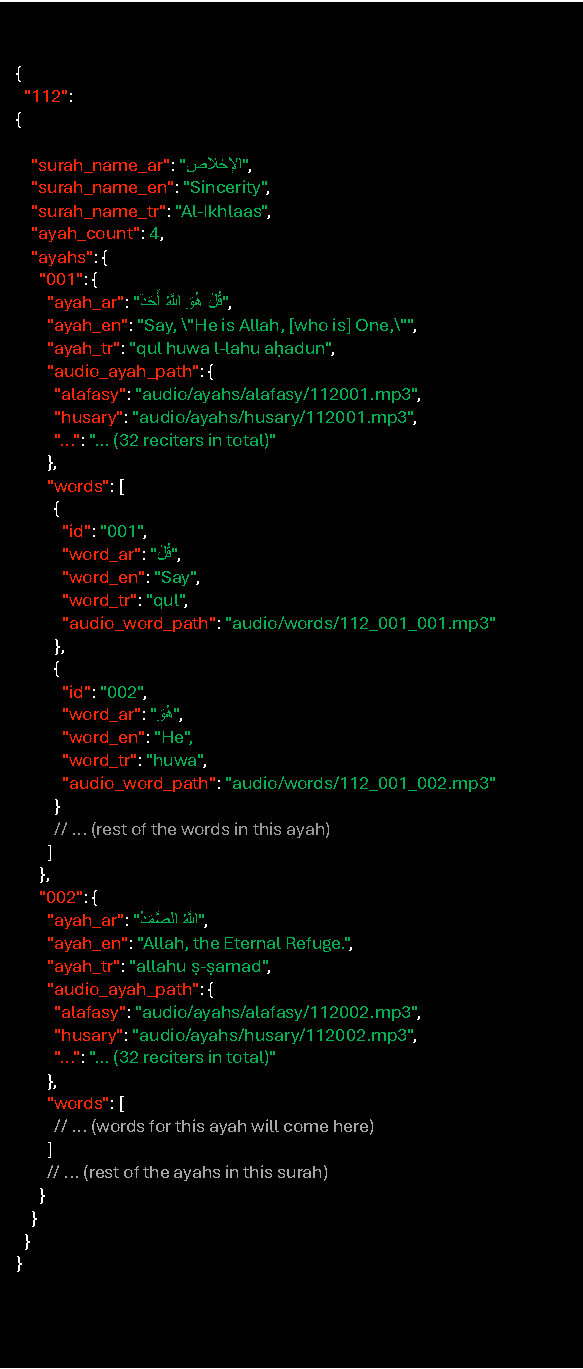
\includegraphics[width=0.31\textwidth]{figures/a.pdf} % Adjust width as needed
    \caption{Example of format of Surah 112 (Al-Ikhlas) in the Dataset.}
    \label{fig:example}
\end{figure}


\begin{table}[ht]
\centering
\caption{Overview of the \textsc{Qur’an-MD} dataset.}
\label{tab:dataset_stats}
\begin{tabular}{@{}lll@{}}
\toprule
\textbf{Category} & \textbf{Attribute} & \textbf{Statistics / Details} \\
\midrule
\multirow{3}{*}{Corpus Size} 
  & Surahs & 114 \\
  & Ayahs & 6,236 \\
  & Words & $\sim$77.8k \\
\addlinespace
\multirow{3}{*}{Audio} 
  & Reciters & 30 (diverse styles) \\
  & Verse-level Audio & $\sim$665 hours \\
  & Word-level Audio & $\sim$22 hours \\
\addlinespace
\multirow{2}{*}{Modalities} 
  & Text & Arabic, English, Transliteration \\
  & Audio & Verse- and Word-level recordings \\
\bottomrule
\end{tabular}
\end{table}





